\begin{frame}
	\frametitle{Escolha do consumidor}

	\begin{itemize}
		\item Um consumidor racional disp\~oe de um presente de \euro 160 para gastar em cal\c cas e em camisas para renovar o seu vestu\'ario.
		\item Uma camisa (bem $x$) custa \euro 20 e um par de cal\c cas (bem $y$) custa \euro 30.
		\item As prefer\^encias podem ser descritas pela fun\c c\~ao $U(x,y)=xy^3$
	\end{itemize}

	\begin{enumerate}
		\item Qual a escolha racional, que maximiza $U$?
		\item Qual a equa\c c\~ao da curva de indiferen\c ca no \'optimo?
	\end{enumerate}

\end{frame}

\begin{frame}
	\frametitle{Escolha do consumidor}

	\onslide<1->{\[U(x,y)=xy^3\]}\\

	\onslide<2->{\[Umg_x = \onslide<3->{y^3}\quad\wedge\quad Umg_y=\onslide<3->{3xy^2}\]}\\

	\onslide<3->{\[\frac{Umg_x}{Umg_y}=\frac{y^3}{3xy^2}=\frac{y}{3x}\]}\\

	\onslide<4->{\[|TMS|=\frac{y}{3x}\]}

\end{frame}

\begin{frame}
	\frametitle{Escolha do consumidor}
	\onslide<1->{
		Restri\c c\~ao Or\c camental: \[30y+20x=160\]
	}

	\onslide<2->{
		De onde podemos encontrar: \[\frac{p_x}{p_y}=\frac{20}{30}=\frac{2}{3}\]
	}

	\onslide<3->{
		E segundo a \onslide<4->{2\textsuperscript{a} lei de Gossen} temos que no \'otimo: \[|TMS|=\frac{p_x}{p_y}\]
	}

	\onslide<5->{
		\[\Rightarrow\quad \frac{y^*}{3x^*} = \frac{2}{3} \quad \Leftrightarrow \quad y^* = 2x^*\]
	}

\end{frame}

\begin{frame}
	\frametitle{Escolha do consumidor}

	Para cumprir com a Restri\c c\~ao Or\c camental, \'e for\c coso que:
	
	\onslide<1->{
		\[30y+20x=160\]
	}

	\onslide<2->{
		\[30\times \overbrace{2x^*}^{y^*=2x^*} + 20x^* = 160\]
	}

	\onslide<3->{
		\[60x^*+20x^*=160 \quad \Leftrightarrow \quad 80x^* = 160\]
	}

	\onslide<4->{
		Ent\~ao $x^*=\frac{160}{80}=2$, e porque $y^*=2x^*$ temos que $y^*=2\times 2 = 4$.

		Assim $U(2,4)=2\times 4^3 = 2\times 64=128$.
	}

\end{frame}

\begin{frame}
	\frametitle{Escolha do consumidor}

	Como no \'optimo $U=128$, ent\~ao podemos encontrar a curva de indifer\^en\c ca:

	\onslide<2->{
		\[U = 128 = xy^3\]
		\[y^3 = \frac{128}{x}\]
		\[y = \left(\frac{128}{x}\right)^{\frac{1}{3}} = \sqrt[3]{\frac{128}{x}}\]
	}

\end{frame}


\begin{frame}
	\frametitle{Escolha do consumidor}
	\begin{center}
		\begin{tikzpicture}[
			scale = 0.8,
			every node/.style={scale = 0.8},
			declare function = {ic(\x) = (128/\x)^(1/3);},
			declare function = {bc(\x) = (16/3) - (2/3)*\x;}
			]

			\draw[->] (-0.1,0) -- (9.1,0)node[below right] {$X$};
			\draw[->] (0,-0.1) -- (0,6.1)node[above left] {$Y$};

			\draw[samples=100,blue,domain=0:(16/2),variable=\x] plot (\x,{bc(\x)});
			
			\draw[samples=100,red,domain=.6:5,variable=\x] plot (\x,{ic(\x)});
			\draw(2,{ic(2)}) node[red,circle,fill,inner sep=1.5pt]{};
			\draw[dashed](2,0) node[below]{$x^*=2$} -- (2,{ic(2)}) -- (0,{ic(2)}) node [left]{$y^*=4$};
		 
		\end{tikzpicture}
	\end{center}
\end{frame}

\begin{frame}
	\frametitle{Custo-Benef\'icio}
	2\textsuperscript{a} Lei de Gossen e escolha \'optima \[\frac{Umg_x}{Umg_y}=\frac{p_x}{p_y}\]

	Consumir mais uma unidade tem um custo marginal \(\frac{p_x}{p_y}\) e um benef\'icio marginal \(\frac{Umg_x}{Umg_y}=|TMS|\)...

	a 2\textsuperscript{a} Lei de Gossen tem impl\'icita a an\'alise custo benef\'icio...
\end{frame}

\begin{frame}
	\frametitle{Dedu\c c\~ao da Procura Individual}
	Iremos considerar uma altera\c c\~ao no pre\c co de mercado de um dos bens e estudar o que acontece aos pontos de escolha \'optima...

	{\color{red}Intui\c c\~ao: se um pre\c co subir, tudo o resto constante, o que acontece \`a quantidade consumida? E porqu\^e?}
\end{frame}

\begin{frame}
	\frametitle{Dedu\c c\~ao da Procura Individual}
	\begin{center}
			Redu\c c\~ao do pre\c co de $x$: $p_x^0>p_x^1>p_x^2$
			\def\rho{0.5}
			\def\ww{15}
			\def\pyy{3}
			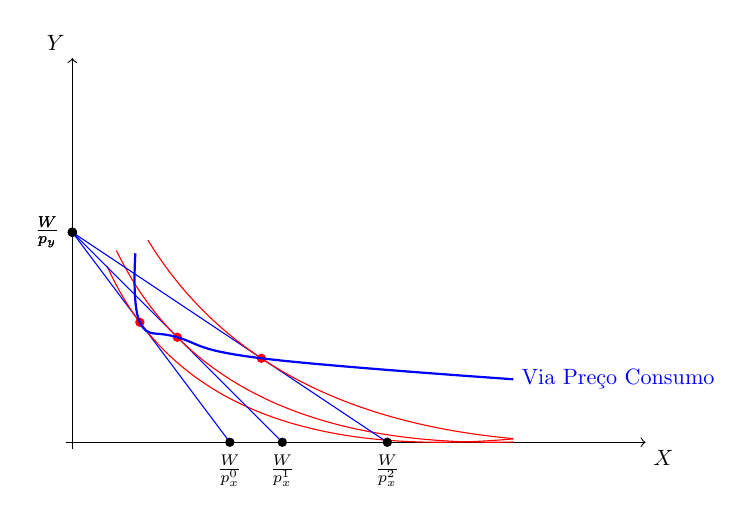
\begin{tikzpicture}[
				scale = 0.8,
				every node/.style={scale = 0.8},
				declare function={
					x(\w,\px,\py) = (\w*(\px^(1/(\rho-1))))/(\px^(\rho/(\rho-1))+\py^(\rho/(\rho-1)));
					y(\w,\px,\py) = (\w*(\py^(1/(\rho-1))))/(\px^(\rho/(\rho-1))+\py^(\rho/(\rho-1)));
					u(\x,\y) = (\x^\rho+\y^\rho)^(1/\rho);
					ic2(\x,\px,\py) = (u(x(\ww,\px,\py),y(\ww,\px,\py))^\rho-\x^\rho)^(1/\rho);
					bc2(\x,\px,\py) = \ww/\py - (\px/\py)*\x;
				}
				]

				\draw[->] (-0.1,0) -- (9.1,0)node[below right] {$X$};
				\draw[->] (0,-0.1) -- (0,6.1)node[above left] {$Y$};


				\onslide<2->{
					\draw[samples=100,blue,domain=0:(\ww/4),variable=\x] plot (\x,{bc2(\x,4,\pyy)});
					\draw({\ww/4},0) node[circle,fill,inner sep=1.5pt,label=below :\(\frac{W}{p_x^0}\)]{};
					\draw(0,{\ww/\pyy}) node[circle,fill,inner sep=1.5pt,label=left :\(\frac{W}{p_y}\)]{};
					\draw[samples=100,red,domain=.55:7,variable=\x] plot (\x,{ic2(\x,4,\pyy)});
					\draw({x(\ww,4,\pyy)},{y(\ww,4,\pyy)}) node[red,circle,fill,inner sep=1.5pt]{};
				}

				\onslide<3->{
					\draw[samples=100,blue,domain=0:(\ww/3),variable=\x] plot (\x,{bc2(\x,3,\pyy)});
					\draw({\ww/3},0) node[circle,fill,inner sep=1.5pt,label=below :\(\frac{W}{p_x^1}\)]{};
					\draw(0,{\ww/\pyy}) node[circle,fill,inner sep=1.5pt,label=left :\(\frac{W}{p_y}\)]{};
					\draw[samples=100,red,domain=.70:7,variable=\x] plot (\x,{ic2(\x,3,\pyy)});
					\draw({x(\ww,3,\pyy)},{y(\ww,3,\pyy)}) node[red,circle,fill,inner sep=1.5pt]{};
				}

				\onslide<4->{
					\draw[samples=100,blue,domain=0:(\ww/2),variable=\x] plot (\x,{bc2(\x,2,\pyy)});
					\draw({\ww/2},0) node[circle,fill,inner sep=1.5pt,label=below :\(\frac{W}{p_x^2}\)]{};
					\draw(0,{\ww/\pyy}) node[circle,fill,inner sep=1.5pt,label=left :\(\frac{W}{p_y}\)]{};
					\draw[samples=100,red,domain=1.2:7,variable=\x] plot (\x,{ic2(\x,2,\pyy)});
					\draw({x(\ww,2,\pyy)},{y(\ww,2,\pyy)}) node[red,circle,fill,inner sep=1.5pt]{};
				}

				\onslide<5->{
					\draw[thick,blue] plot[smooth, tension=0.7] coordinates{(1,3) ({x(\ww,4,\pyy)},{y(\ww,4,\pyy)}) ({x(\ww,3,\pyy)},{y(\ww,3,\pyy)}) ({x(\ww,2,\pyy)},{y(\ww,2,\pyy)}) (7,1)} node[right]{Via Pre\c co Consumo};
				}

			\end{tikzpicture}
		\end{center}
\end{frame}

\begin{frame}
	\frametitle{Dedu\c c\~ao da Procura Individual - Curva Pre\c co Consumo}
	\begin{center}
			Redu\c c\~ao do pre\c co de $x$: $p_x^0>p_x^1>p_x^2$

			\def\rho{0.5}
			\def\ww{15}
			\def\pyy{3}
			\begin{tikzpicture}[
				scale = 0.8,
				every node/.style={scale = 0.8},
				declare function={
					x(\w,\px,\py) = (\w*(\px^(1/(\rho-1))))/(\px^(\rho/(\rho-1))+\py^(\rho/(\rho-1)));
					y(\w,\px,\py) = (\w*(\py^(1/(\rho-1))))/(\px^(\rho/(\rho-1))+\py^(\rho/(\rho-1)));
					u(\x,\y) = (\x^\rho+\y^\rho)^(1/\rho);
					ic2(\x,\px,\py) = (u(x(\ww,\px,\py),y(\ww,\px,\py))^\rho-\x^\rho)^(1/\rho);
					bc2(\x,\px,\py) = \ww/\py - (\px/\py)*\x;
				}
				]

				\draw[->] (-0.1,0) -- (9.1,0)node[below right] {$X$};
				\draw[->] (0,-0.1) -- (0,6.1)node[above left] {$Y$};

				\draw({x(\ww,4,\pyy)},{y(\ww,4,\pyy)}) node[red,circle,fill,inner sep=1.5pt,label=above:\(p_x^0\)]{};
				\draw({x(\ww,3,\pyy)},{y(\ww,3,\pyy)}) node[red,circle,fill,inner sep=1.5pt,label=above:\(p_x^1\)]{};
				\draw({x(\ww,2,\pyy)},{y(\ww,2,\pyy)}) node[red,circle,fill,inner sep=1.5pt,label=above:\(p_x^2\)]{};

				\draw[thick,blue] plot[smooth, tension=0.7] coordinates{(1,3) ({x(\ww,4,\pyy)},{y(\ww,4,\pyy)}) ({x(\ww,3,\pyy)},{y(\ww,3,\pyy)}) ({x(\ww,2,\pyy)},{y(\ww,2,\pyy)}) (7,1)};

			\end{tikzpicture}
		\end{center}
\end{frame}

\begin{frame}
	\frametitle{Dedu\c c\~ao da Procura Individual}
	N\~ao h\'a raz\~ao para assumir que a Curva de Pre\c co Consumo tem uma forma est\'andar (crescente, descrescente, etc). O que vai determinar o que se passa perante um cambio no pre\c co de $x$ s\~ao as prefer\^encias. A Curva Pre\c co Consumo tamb\'em \'e conhecida como Offer Curve.\pause

	O que sabemos \'e que n\~ao pode ir para acima de\pause $\frac{W}{p_y}$.
\end{frame}

\begin{frame}
	\frametitle{Dedu\c c\~ao da Procura Individual}
	\begin{center}

			\def\rho{0.5}
			\def\ww{15}
			\def\pyy{3}
			\begin{tikzpicture}[
				scale = 0.4,
				every node/.style={scale = 0.5},
				declare function={
					x(\w,\px,\py) = (\w*(\px^(1/(\rho-1))))/(\px^(\rho/(\rho-1))+\py^(\rho/(\rho-1)));
					y(\w,\px,\py) = (\w*(\py^(1/(\rho-1))))/(\px^(\rho/(\rho-1))+\py^(\rho/(\rho-1)));
					u(\x,\y) = (\x^\rho+\y^\rho)^(1/\rho);
					ic2(\x,\px,\py) = (u(x(\ww,\px,\py),y(\ww,\px,\py))^\rho-\x^\rho)^(1/\rho);
					bc2(\x,\px,\py) = \ww/\py - (\px/\py)*\x;
				}
				]

				\draw[->] (-0.1,0) -- (9.1,0)node[below right] {$X$};
				\draw[->] (0,-0.1) -- (0,6.1)node[above left] {$Y$};

				\draw({x(\ww,4,\pyy)},{y(\ww,4,\pyy)}) node[red,circle,fill,inner sep=1.5pt,label=above:\(p_x^0\)]{};
				\draw({x(\ww,3,\pyy)},{y(\ww,3,\pyy)}) node[red,circle,fill,inner sep=1.5pt,label=above:\(p_x^1\)]{};
				\draw({x(\ww,2,\pyy)},{y(\ww,2,\pyy)}) node[red,circle,fill,inner sep=1.5pt,label=above:\(p_x^2\)]{};

				\draw[blue] plot[smooth, tension=0.7] coordinates{(1,3.5) ({x(\ww,4,\pyy)},{y(\ww,4,\pyy)}) ({x(\ww,3,\pyy)},{y(\ww,3,\pyy)}) ({x(\ww,2,\pyy)},{y(\ww,2,\pyy)}) (6,1)};

				\onslide<2->{
					\draw[->] (-0.1,-8) -- (9.1,-8)node[below right] {$X$};
					\draw[->] (0,-8.1) -- (0,-1.9)node[above left] {$p_x$};

					\draw[dotted] ({x(\ww,4,\pyy)},{y(\ww,4,\pyy)}) -- ({x(\ww,4,\pyy)},-8);
					\draw[dotted] ({x(\ww,3,\pyy)},{y(\ww,3,\pyy)}) -- ({x(\ww,3,\pyy)},-8);
					\draw[dotted] ({x(\ww,2,\pyy)},{y(\ww,2,\pyy)}) -- ({x(\ww,2,\pyy)},-8);
				}

				\onslide<3->{
					\draw[dotted] (0,{4-8})node[left]{\(p_x^0\)} -- ({x(\ww,4,\pyy)},{4-8});
					\draw[dotted] (0,{3-8})node[left]{\(p_x^1\)} -- ({x(\ww,3,\pyy)},{3-8});
					\draw[dotted] (0,{2-8})node[left]{\(p_x^2\)} -- ({x(\ww,2,\pyy)},{2-8});
			 	}

			 	\onslide<4->{
			 		\draw[thick,green] plot[smooth,tension=0.4] coordinates{(1,-3.5) ({x(\ww,4,\pyy)},{4-8}) ({x(\ww,3,\pyy)},{3-8}) ({x(\ww,2,\pyy)},{2-8}) (6,-6.5)} node[black,below right]{\parbox[l]{4cm}{Curva de Procura Individual pelo bem \(x\)}};
			 	}

			\end{tikzpicture}
		\end{center}
\end{frame}

\begin{frame}
	\frametitle{Curva da Procura}
	\'E o conjunto dos pares $(Q,P)$ de escolha \'optima, para diferentes pre\c cos, dado um valor fixo para as vari\'aveis ex\'ogenas \`as decis\~oes do consumidor:\pause
	\begin{itemize}
		\item Rendimento dispon\'ivel\pause
		\item Pre\c co dos outros bens\pause
		\item Prefer\^encias e factores que as influenciem
	\end{itemize}
\end{frame}

\begin{frame}
	\frametitle{Lei da Procura}
	Entre a quantidade procurada de um bem e o pre\c co desse mesmo bem, existe uma rela\c c\~ao negativa: 
	\begin{tcolorbox}[colback=iscal_color!10,colframe=iscal_color]
		Se o pre\c co aumenta, a quantidade procurada diminui, \emph{c\ae teris paribus}
	\end{tcolorbox}

	\footnotesize{Aten\c c\~ao: dada a altera\c c\~ao de pre\c co, trata-se de uma altera\c c\~ao da quantidade, ou seja, das inten\c c\~oes de consumo/compra...}
\end{frame}

\begin{frame}
	\frametitle{A Lei da Procura}
	\begin{center}
		\begin{tikzpicture}[
			scale = 1,
			every node/.style={scale = 1},
			declare function = {d1(\x) = 6-1.3*(\x^(0.8));}
		]

		\draw[->] (-0.1,0) -- (6.1,0)node[below right] {$X$};
		\draw[->] (0,-0.1) -- (0,6.1)node[above left] {$p_x$};

		\onslide<2->{
			\draw[blue,thick,domain=0.6:5.4,variable=\x,samples=100] plot (\x,{d1(\x)});
			\draw(5.4,{d1(5.4)}) node[right]{\(D\)};
		}

		\onslide<3->{
			\draw[dashed] (4,0) node[below]{4} -- (4,{d1(4)}) node[circle,fill,inner sep=1.5pt,label=above right:$a$]{} -- (0,{d1(4)}) node[left]{2};
		}

		\onslide<4->{
			\draw(0,{d1(3)}) node[left]{3};
			\draw[thick,red,->](0,{d1(4)}) -- (0,{d1(3)});
		}

		\onslide<5->{
			\draw[dashed] (3,0) node[below]{3} -- (3,{d1(3)}) node[circle,fill,inner sep=1.5pt,label=above right:$b$]{} -- (0,{d1(3)}) node[left]{3};
			\draw[->,thick,red] (4,{d1(4)}) -- (3,{d1(3)});
			\draw[->,thick,red] (4,0) -- (3,0);
		}

		\end{tikzpicture}
	\end{center}
\end{frame}

\begin{frame}
	\frametitle{Curva de Procura}
	Mudan\c cas no \textbf{pre\c co} v\~ao causar movimentos \textbf{ao longo} da curva de procura.

	\vspace{0.4cm}

	\'E importante distinguir entre mudan\c cas na procura, de mudan\c cas na \emph{quantidade procurada}.

	\vspace{0.4cm}

	Quando definimos a procura, temos quantidade procurada para um pre\c co, ou seja a quantidade \'e fun\c c\~ao do pre\c co, $Q_x=f(p_x)$.

	\vspace{0.4cm}

	Assim, no nosso gr\'afico temos ao contr\'ario, ou seja tempos o pre\c co associado \'a um n\'ivel de quantidade procurada, ou seja $P=g(Q_x)$. Esta curva de procura tambem \'e conhecida como \textbf{procura inversa}. Isto \'e, na verdade, a mesma coisa que a procura s\'o que vista desde um ponto de vista diferente.

\end{frame}

\begin{frame}
	\frametitle{Procura}

	Se a altera\c c\~ao de um pre\c co, \emph{caeteris paribus}, leva a uma altera\c c\~ao de um ponto para outro na mesma curva de procura, ent\~ao o que faz alterar a posi\c c\~ao da curva?!?

\end{frame}

\begin{frame}
	\frametitle{Que vari\'aveis afectam a Procura?}
	A quantidade de um bem que os consumidores adquirir depende de:

	\begin{columns}
		\begin{column}{0.65\textwidth}
			\begin{itemize}
				\item \(p =\) pre\c co de adquisi\c c\~ao {\color{red}(-)}
					\begin{itemize}
						\item Na mesma curva, passase para outro ponto
					\end{itemize}
				\item \(p_r =\) pre\c co de bens relacionados no consumo:
					\begin{itemize}
						\item Bens substitutos {\color{red}(+)}
						\item Bens complement\'arios {\color{red}(-)}
					\end{itemize}
				\item \(W=\) rendimento dispon\'ivel para consumo
					\begin{itemize}
						\item Bem normal {\color{red}(+)}
						\item Bem inferior {\color{red}(-)}
					\end{itemize}
				\item Prefer\^encias e factores que as afectem
			\end{itemize}
		\end{column}
		\begin{column}{0.3\textwidth}
			\onslide<2->{
			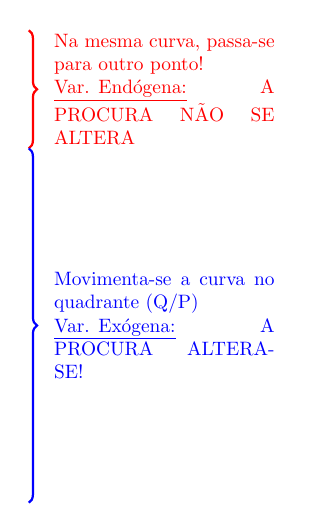
\begin{tikzpicture}[
				scale = 1,
				every node/.style = {scale = 0.7}
				]
				\draw [decorate,decoration={brace,mirror,amplitude=3pt},thick,red] (0,3.5) -- (0,5) node [midway,xshift=70pt] {\parbox{4cm}{Na mesma curva, passa-se para outro ponto!\\ \underline{Var. End\'ogena:} A PROCURA N\~AO SE ALTERA}};
				
				\draw [decorate,decoration={brace,mirror,amplitude=3pt},thick,blue] (0,-1) -- (0,3.5) node [midway,xshift=70pt] {\parbox{4cm}{Movimenta-se a curva no quadrante (Q/P)\\ \underline{Var. Ex\'ogena:} A PROCURA ALTERA-SE!}};
			\end{tikzpicture}
			}
		\end{column}
	\end{columns}

\end{frame}

\begin{frame}
	\frametitle{Classifica\c c\~ao entre bens dada a sua rela\c c\~ao de consumo}
	\begin{itemize}
		\item Bens substitutos
		\begin{itemize}
			\item Altera\c c\~oes no pre\c co de um dos bens implicam varia\c c\~oes no mesmo sentido na procura do outro bem.
			\item Quando o pre\c co de um bem aumenta, a procura do outro bem aumenta
		\end{itemize}
		\item Bens complementares
		\begin{itemize}
			\item Altera\c c\~oes no pre\c co de um dos bens implicam varia\c c\~oes no sentido oposto na procura do outro bem
			\item Quando o pre\c co de um aumenta, a procura do outro diminui.
		\end{itemize}
	\end{itemize}
\end{frame}

\begin{frame}
	\frametitle{Classifica\c c\~ao entre bens dada a sua rela\c c\~ao com o rendimento}
	\begin{itemize}
		\item Bem normal
		\begin{itemize}
			\item A sua procura aumenta quando o rendimento aumenta
			\item Aumentos no rendimento deslocam a curva de procura para a direita
		\end{itemize}
		\item Bem inferior
		\begin{itemize}
			\item Aumentos no rendimento fazem diminuir a sua procura
			\item Aumento no rendimento faz a curva deslocar-se para a esquerda
		\end{itemize}
	\end{itemize}
\end{frame}

\begin{frame}
	\frametitle{Procura}
	\begin{itemize}
		\item \`A rela\c c\~ao funcional entre a quantidade procurada de um bem e todas as vari\'aveis que a infuienciam, chama-se \underline{Fun\c c\~ao Procura}: \[Q_d=f(p,p_r,W,...)\]
		\item A curva de procura obt\'em-se estudando a rela\c c\~ao que existe entre a quantidade procurada, {\color{red}\(Q_D\)}, e o seu pre\c co, {\color{red}\(p\)}, para valores \textbf{dados} das outras vari\'aveis.

		{\small (que n\~ao est\~ao representadas nos eixos, onde se representa o gr\'afico da Procura)}
	\end{itemize}
\end{frame}

\begin{frame}
	\frametitle{Expans\~ao da Procura}
	Que altera\c c\~ao de vari\'aveis ex\'ogenas poderia estar na origem da desloca\c c\~ao da procura?
	\begin{center}
		\begin{tikzpicture}[
			scale = 1,
			every node/.style={scale = 1},
			declare function = {
				d1(\x) = 5.5-1.3*(\x^(0.8));
				d2(\x) = 6.5-1.3*(\x^(0.8));
			}
		]

		\draw[->] (-0.1,0) -- (6.1,0)node[below right] {$X$};
		\draw[->] (0,-0.1) -- (0,6.1)node[above left] {$p_x$};
		\draw[blue,thick,domain=0.6:5.4,variable=\x,samples=100] plot (\x,{d1(\x)}) node[right]{D};
		\draw[dashed] (3,0) node[below]{3} -- (3,{d1(3)}) node[circle,fill,inner sep=1.5pt,label=below left:$b$]{} -- (0,{d1(3)}) node[left]{3};
		
		\onslide<2->{
			\draw[red,thick,domain=0.6:5.4,variable=\x,samples=100] plot (\x,{d2(\x)}) node[right]{\(D'\)};
		}

		\onslide<3-4>{
			\draw[thick,blue,->] (3,{d1(3)}) -- (3,{d2(3)});
		}

		\only<4>{
			\draw[thick,blue,->] (3,{d1(3)}) -- (4.2,{d1(3)});
		}

		\end{tikzpicture}
	\end{center}
\end{frame}

\begin{frame}
	\frametitle{Expans\~ao da Procura}
	Que altera\c c\~ao de vari\'aveis ex\'ogenas poderia estar na origem da desloca\c c\~ao da procura?
	\begin{center}
		\begin{tikzpicture}[
			scale = 1,
			every node/.style={scale = 1},
			declare function = {
				d1(\x) = 5.5-1.3*(\x^(0.8));
				d2(\x) = 6.5-1.3*(\x^(0.8));
			}
		]

		\draw[->] (-0.1,0) -- (6.1,0)node[below right] {$X$};
		\draw[->] (0,-0.1) -- (0,6.1)node[above left] {$p_x$};
		
		\onslide<2->{
			\draw[red,thick,domain=0.6:5.4,variable=\x,samples=100] plot (\x,{d1(\x)}) node[right]{\(D'\)};
			
		}

		\onslide<1->{
			\draw[blue,thick,domain=0.6:5.4,variable=\x,samples=100] plot (\x,{d2(\x)}) node[right]{\(D\)};
			\draw[dashed] (3,0) node[below]{3} -- (3,{d2(3)}) node[circle,fill,inner sep=1.5pt,label=above right:$b$]{} -- (0,{d2(3)}) node[left]{3};
		}

		\onslide<3-4>{
			\draw[thick,blue,<-] (3,{d1(3)}) -- (3,{d2(3)});
		}

		\only<4>{
			\draw[thick,blue,<-] (2,{d2(3)}) -- (3,{d2(3)});
		}

		\end{tikzpicture}
	\end{center}
\end{frame}

\begin{frame}
	\frametitle{Classifica\c c\~ao de Bens}
	Em fun\c c\~ao de uma altera\c c\~ao de rendimento, \emph{c\ae teris paribus}:
	\begin{itemize}
		\item Bens normais - $Q^d$ varia no mesmo sentido de $W$
		\item Bens inferiores - $Q^d$ varia inversamente a $W$
	\end{itemize}
\end{frame}

\begin{frame}
	\frametitle{Aumento de rendimento}
	\begin{columns}
		\begin{column}{0.47\textwidth}
			\begin{tikzpicture}[
				scale = .7,
				every node/.style = {scale = .7},
				declare function = {d0(\x)=6-1.2*(\x*(0.9));},
				declare function = {d1(\x)=6-1.2*((\x-1)^(0.9));}
			]

			\draw[->] (-0.1,0) -- (6.1,0)node[below] {$X$};
			\draw[->] (0,-0.1) -- (0,6.1)node[left] {$p_x$};

			\draw[domain=1:5,variable=\x,samples=100] plot (\x,{d0(\x)});
			\draw[domain=1:5,variable=\x,samples=100,red] plot (\x,{d1(\x)});

			\draw[<-,blue,thick] (3,{d1(3)}) -- (2,{d1(3)});

			\draw(4,{d1(4)}) node[right,red]{$D_1$};
			\draw(4,{d0(4)}) node[left]{$D_0$};

			\end{tikzpicture}

			Para um bem normal, expans\~ao da Procura
		\end{column}
		\begin{column}{0.47\textwidth}
		\begin{tikzpicture}[
				scale = .7,
				every node/.style = {scale = .7},
				declare function = {d0(\x)=6-1.2*(\x*(0.9));},
				declare function = {d1(\x)=6-1.2*((\x-1)^(0.9));}
			]

			\draw[->] (-0.1,0) -- (6.1,0)node[right] {$X$};
			\draw[->] (0,-0.1) -- (0,6.1)node[left] {$p_x$};

			\draw[domain=1:5,variable=\x,samples=100,red] plot (\x,{d0(\x)});
			\draw[domain=1:5,variable=\x,samples=100] plot (\x,{d1(\x)});

			\draw[->,blue,thick] (3,{d1(3)}) -- (2,{d1(3)});

			\draw(4,{d1(4)}) node[right]{$D_0$};
			\draw(4,{d0(4)}) node[left,red]{$D_1$};

			\end{tikzpicture}
			Para um bem inferior, contrac\c c\~ao da Procura
		\end{column}
	\end{columns}
\end{frame}

\begin{frame}
	\frametitle{Dedu\c c\~ao da Procura Individual}
	\begin{center}

			\def\rho{0.5}
			\def\ww{10}
			\def\whw{22}
			\def\pyy{3}
			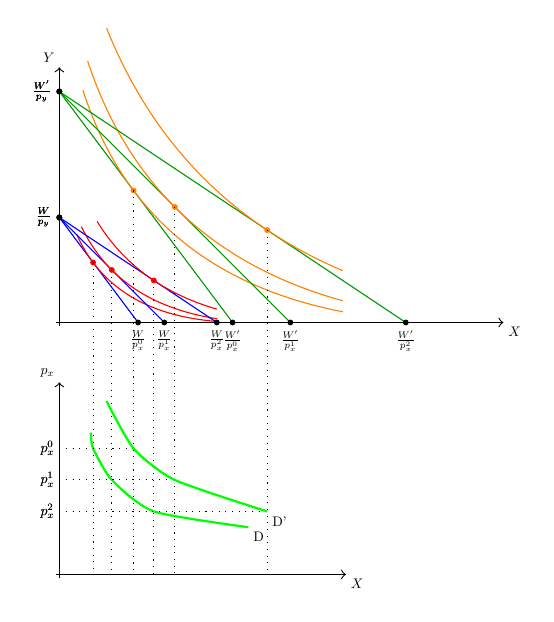
\begin{tikzpicture}[
				scale = 0.4,
				every node/.style={scale = 0.5},
				declare function={
					x(\w,\px,\py) = (\w*(\px^(1/(\rho-1))))/(\px^(\rho/(\rho-1))+\py^(\rho/(\rho-1)));
					y(\w,\px,\py) = (\w*(\py^(1/(\rho-1))))/(\px^(\rho/(\rho-1))+\py^(\rho/(\rho-1)));
					u(\x,\y) = (\x^\rho+\y^\rho)^(1/\rho);
					ic2(\x,\px,\py) = (u(x(\ww,\px,\py),y(\ww,\px,\py))^\rho-\x^\rho)^(1/\rho);
					bc2(\x,\px,\py) = \ww/\py - (\px/\py)*\x;
					ic3(\x,\px,\py) = (u(x(\whw,\px,\py),y(\whw,\px,\py))^\rho-\x^\rho)^(1/\rho);
					bc3(\x,\px,\py) = \whw/\py - (\px/\py)*\x;
				}
				]

				\draw[->] (-0.1,0) -- (14.1,0)node[below right] {$X$};
				\draw[->] (0,-0.1) -- (0,8.1)node[above left] {$Y$};

				\draw[samples=100,blue,domain=0:(\ww/4),variable=\x] plot (\x,{bc2(\x,4,\pyy)});
				\draw({\ww/4},0) node[circle,fill,inner sep=1.5pt,label=below :\(\frac{W}{p_x^0}\)]{};
				\draw(0,{\ww/\pyy}) node[circle,fill,inner sep=1.5pt,label=left :\(\frac{W}{p_y}\)]{};
				\draw[samples=100,red,domain=.55:5,variable=\x] plot (\x,{ic2(\x,4,\pyy)});
				\draw({x(\ww,4,\pyy)},{y(\ww,4,\pyy)}) node[red,circle,fill,inner sep=1.5pt]{};

				\draw[samples=100,blue,domain=0:(\ww/3),variable=\x] plot (\x,{bc2(\x,3,\pyy)});
				\draw({\ww/3},0) node[circle,fill,inner sep=1.5pt,label=below :\(\frac{W}{p_x^1}\)]{};
				\draw(0,{\ww/\pyy}) node[circle,fill,inner sep=1.5pt,label=left :\(\frac{W}{p_y}\)]{};
				\draw[samples=100,red,domain=.70:5,variable=\x] plot (\x,{ic2(\x,3,\pyy)});
				\draw({x(\ww,3,\pyy)},{y(\ww,3,\pyy)}) node[red,circle,fill,inner sep=1.5pt]{};

				\draw[samples=100,blue,domain=0:(\ww/2),variable=\x] plot (\x,{bc2(\x,2,\pyy)});
				\draw({\ww/2},0) node[circle,fill,inner sep=1.5pt,label=below :\(\frac{W}{p_x^2}\)]{};
				\draw(0,{\ww/\pyy}) node[circle,fill,inner sep=1.5pt,label=left :\(\frac{W}{p_y}\)]{};
				\draw[samples=100,red,domain=1.2:5,variable=\x] plot (\x,{ic2(\x,2,\pyy)});
				\draw({x(\ww,2,\pyy)},{y(\ww,2,\pyy)}) node[red,circle,fill,inner sep=1.5pt]{};

				\draw[->] (-0.1,-8) -- (9.1,-8)node[below right] {$X$};
				\draw[->] (0,-8.1) -- (0,-1.9)node[above left] {$p_x$};

				\onslide<1-2>{

					\draw[dotted] ({x(\ww,4,\pyy)},{y(\ww,4,\pyy)}) -- ({x(\ww,4,\pyy)},-8);
					\draw[dotted] ({x(\ww,3,\pyy)},{y(\ww,3,\pyy)}) -- ({x(\ww,3,\pyy)},-8);
					\draw[dotted] ({x(\ww,2,\pyy)},{y(\ww,2,\pyy)}) -- ({x(\ww,2,\pyy)},-8);

					\draw[dotted] (0,{4-8})node[left]{\(p_x^0\)} -- ({x(\ww,4,\pyy)},{4-8});
					\draw[dotted] (0,{3-8})node[left]{\(p_x^1\)} -- ({x(\ww,3,\pyy)},{3-8});
					\draw[dotted] (0,{2-8})node[left]{\(p_x^2\)} -- ({x(\ww,2,\pyy)},{2-8});

				}

		 		\draw[thick,green] plot[smooth,tension=0.4] coordinates{(1,-3.5) ({x(\ww,4,\pyy)},{4-8}) ({x(\ww,3,\pyy)},{3-8}) ({x(\ww,2,\pyy)},{2-8}) (6,-6.5)} node[black,below right]{D};

		 		\onslide<2->{

			 		\draw[samples=100,green!60!black,domain=0:(\whw/4),variable=\x] plot (\x,{bc3(\x,4,\pyy)});
					\draw({\whw/4},0) node[circle,fill,inner sep=1.5pt,label=below :\(\frac{W'}{p_x^0}\)]{};
					\draw(0,{\whw/\pyy}) node[circle,fill,inner sep=1.5pt,label=left :\(\frac{W'}{p_y}\)]{};
					\draw[samples=100,orange,domain=.75:9,variable=\x] plot (\x,{ic3(\x,4,\pyy)});
					\draw({x(\whw,4,\pyy)},{y(\whw,4,\pyy)}) node[orange,circle,fill,inner sep=1.5pt]{};

					\draw[samples=100,green!60!black,domain=0:(\whw/3),variable=\x] plot (\x,{bc3(\x,3,\pyy)});
					\draw({\whw/3},0) node[circle,fill,inner sep=1.5pt,label=below :\(\frac{W'}{p_x^1}\)]{};
					\draw(0,{\whw/\pyy}) node[circle,fill,inner sep=1.5pt,label=left :\(\frac{W'}{p_y}\)]{};
					\draw[samples=100,orange,domain=.90:9,variable=\x] plot (\x,{ic3(\x,3,\pyy)});
					\draw({x(\whw,3,\pyy)},{y(\whw,3,\pyy)}) node[orange,circle,fill,inner sep=1.5pt]{};

					\draw[samples=100,green!60!black,domain=0:(\whw/2),variable=\x] plot (\x,{bc3(\x,2,\pyy)});
					\draw({\whw/2},0) node[circle,fill,inner sep=1.5pt,label=below :\(\frac{W'}{p_x^2}\)]{};
					\draw(0,{\whw/\pyy}) node[circle,fill,inner sep=1.5pt,label=left :\(\frac{W'}{p_y}\)]{};
					\draw[samples=100,orange,domain=1.5:9,variable=\x] plot (\x,{ic3(\x,2,\pyy)});
					\draw({x(\whw,2,\pyy)},{y(\whw,2,\pyy)}) node[orange,circle,fill,inner sep=1.5pt]{};

		 		}

		 		\onslide<3->{

		 			\draw[dotted] ({x(\whw,4,\pyy)},{y(\whw,4,\pyy)}) -- ({x(\whw,4,\pyy)},-8);
					\draw[dotted] ({x(\whw,3,\pyy)},{y(\whw,3,\pyy)}) -- ({x(\whw,3,\pyy)},-8);
					\draw[dotted] ({x(\whw,2,\pyy)},{y(\whw,2,\pyy)}) -- ({x(\whw,2,\pyy)},-8);

					\draw[dotted] (0,{4-8})node[left]{\(p_x^0\)} -- ({x(\whw,4,\pyy)},{4-8});
					\draw[dotted] (0,{3-8})node[left]{\(p_x^1\)} -- ({x(\whw,3,\pyy)},{3-8});
					\draw[dotted] (0,{2-8})node[left]{\(p_x^2\)} -- ({x(\whw,2,\pyy)},{2-8});

			 		\draw[thick,green] plot[smooth,tension=0.4] coordinates{(1.5,-2.5) ({x(\whw,4,\pyy)},{4-8}) ({x(\whw,3,\pyy)},{3-8}) ({x(\whw,2,\pyy)},{2-8})} node[black,below right]{D'};

		 		}

			\end{tikzpicture}
		\end{center}
\end{frame}

\begin{frame}
	\frametitle{Curva de Procura}
	\begin{itemize}
		\item Da determina\c c\~ao do \'optimo do consumidor, deduz-se, ent\~ao, a procura individual
		\item {\color{red} Por adi\c c\~ao}, obt\'em-se {\color{red}a procura de mercado}, que herda todas as propriedades das procuras individuais
	\end{itemize}
	\[Q^D(P)=\sum_{i=1}^n Q^D_i(P)\]
\end{frame}

\begin{frame}
	\frametitle{Modelos Lineares para a Procura}
	Para a simplifica\c c\~ao de c\'alculo, \'e frequente utilizar-se modelos lineares para a Procura, na forma:
	\begin{itemize}
		\item \(Q=a-b\times P\) (forma directa)
		\item \(P=\frac{a}{b}-\frac{1}{b}Q\) (forma inversa)
	\end{itemize}
	\vspace{1cm}
	{\small \color{red} Seja qual for a forma, representa-se sempre no espa\c co \((Q,P)\), devido a Marshall (1895) ``Principles of Economics''}
\end{frame}

\begin{frame}
	\frametitle{Alfred Marshall}
	\begin{center}
		\includegraphics[width=0.5\textwidth]{Alfred_Marshall.jpg}
	\end{center}
\end{frame}

\begin{frame}
	\frametitle{Modelos Lineares para a Procura: Interpreta\c c\~oes}
	\begin{center}
		\begin{tikzpicture}[
			scale = .8,
			every node/.style = {scale=.8},
			declare function = {d(\x)=4-\x;}
		]

			\draw[->] (-0.1,0) -- (5.1,0)node[below right] {$X$};
			\draw[->] (0,-0.1) -- (0,5.1)node[above left] {$p_x$};

			\draw[blue,thick,domain=0:4,variable=\x] plot (\x,{d(\x)});
			\draw(0,4) node[left]{$\frac{a}{b}$};
			\draw(4,0) node[below]{$a$};

			\draw[dashed](2,0) node[below]{$q_1$} -- (2,{d(2)})node[circle,fill,inner sep=1.5pt]{} -- (0,{d(2)}) node[left]{$p_1$};

			\draw(3,1) node[above right]{$D$};
			\draw(3,3) node[above]{$q=a-b\times p$};

		\end{tikzpicture}
	\end{center}

	Para adquirir $q_1$, no m\'aximo os consumidores est\~ao dispostos a pagar $p_1$ por unidade... ou

	Ao pre\c co $p_1$, a escolha \'optima de consumo \'e $q_1$ (individual ou somat\'orio das individuais...)

\end{frame}

\begin{frame}
	\frametitle{Modelos Lineares para a Procura: Interpreta\c c\~oes}
	\begin{center}
		\begin{tikzpicture}[
			scale = .8,
			every node/.style = {scale=.8},
			declare function = {d(\x)=4-\x;}
		]

			\draw[->] (-0.1,0) -- (5.1,0)node[below right] {$X$};
			\draw[->] (0,-0.1) -- (0,5.1)node[above left] {$p_x$};

			\draw[blue,thick,domain=0:4,variable=\x] plot (\x,{d(\x)});
			\draw(0,4) node[left]{$\frac{a}{b}$};
			\draw(4,0) node[below]{$a$};

			\draw[dashed](2,0) node[below]{$q_1$} -- (2,{d(2)})node[circle,fill,inner sep=1.5pt]{} -- (0,{d(2)}) node[left]{$p_1$};

			\draw(3,1) node[above right]{$D$};
			\draw(3,3) node[above]{$q=a-b\times p$};

			\only<2>{
				\draw[red,fill](0,0) -- (2,0) -- (2,{d(2)}) -- (0,{d(2)}) -- (0,0);
			}
			\only<3>{
				\draw[green,fill](0,{d(2)}) -- (0,4) -- (2,{d(2)}) -- (0,{d(2)});
			}

		\end{tikzpicture}
	\end{center}
	{\footnotesize
	\begin{itemize}
		\item $p_1\times q_1$ corresponde \'a {\color{red} despesa} de consumo do bem em an\'alise;
		\item $\left(\frac{a}{b}-p_1\right)\times q_1 \times\frac{1}{2}$ corresponde ao {\color{green} excedente} do consumidor, ou seja corresponde \`a \'area do triangulo acima de $p_1$ e abaixo da Procura.
	\end{itemize}
	}
\end{frame}

\begin{frame}
	\frametitle{Excedente do Consumidor}
	Por unidade do bem transaccionado, \'e a diferen\c ca entre o que o consumidor paga por unidade e o m\'aximo que estaria disposto a pagar (pre\c co de reserva, dado pela procura inversa)...

	\vspace{1cm}

	O excedente total do consumidor num mecado \'e o somat\'orio de todos os excedentes individuais e corresponde graficamente \`a \'area abaixo da curva de procura e acima do pre\c co de mercado.
\end{frame}